% !TeX root = ../main.tex

\chapter{结果与讨论}
\section{图表数据}
分析数据,得如下表\ref{tab3.1}-\ref{tab3.2}.
\begin{figure}[htbp]
  \begin{floatrow}[3]
    \tablebox{\caption{室温}}{%
      \label{tab3.1}
      \begin{tabular}{cc}
        \toprule
        $t$   & $T$/\si{\degreeCelsius}  \\
        \midrule
        14:33	&	21.5		\\
        15:54	&	21.0		\\
        16:55	&	19.8		\\
        $\overline{t}$ &20.77\\
        \bottomrule
      \end{tabular}
    }%
    \tablebox{\caption{最大吸光度与光波长对照表}}{%
      \label{tab3.2}
      \begin{tabular}{cc}
        \toprule
        $\lambda_\text{max} $   & $D_\text{max}$  \\
        \midrule
        ——	&	0.002 	\\
        439.00 	&	0.209 	\\
        440.80 	&	0.193 	\\
        591.60 	&	0.187 	\\
        591.60 	&	0.249 	\\
        591.60 	&	0.393 	\\
        591.80 	&	0.461 	\\
        591.60 	&	0.514 	\\
        590.20 	&	0.642 	\\
        436.20 	&	0.231 	\\
        \bottomrule
      \end{tabular}
    }%
    \tablebox{\caption{室温}}{%
    \label{tab3.3}
    \begin{tabular}{ccc}
      \toprule
      pH   & $\frac{D-D_1}{D_2-D}$ & $\lg\frac{D-D_1}{D_2-D}$ \\
      \midrule
      3.210 	&	-0.051 	&	\#NUM!	\\
      3.420 	&	-0.085 	&	\#NUM!	\\
      3.660 	&	-0.097 	&	\#NUM!	\\
      3.800 	&	0.046 	&	-1.339 	\\
      4.190 	&	0.651 	&	-0.187 	\\
      4.380 	&	1.271 	&	0.104 	\\
      4.580 	&	2.211 	&	0.345 	\\
      \bottomrule
    \end{tabular}
  }
  \end{floatrow}
\end{figure}

求出$\lg\frac{D-D_1}{D_2-D}$,如上表\ref{tab3.3},由pH对其作图,得下图\ref{fig1}

\begin{figure}[h]
  \centering
  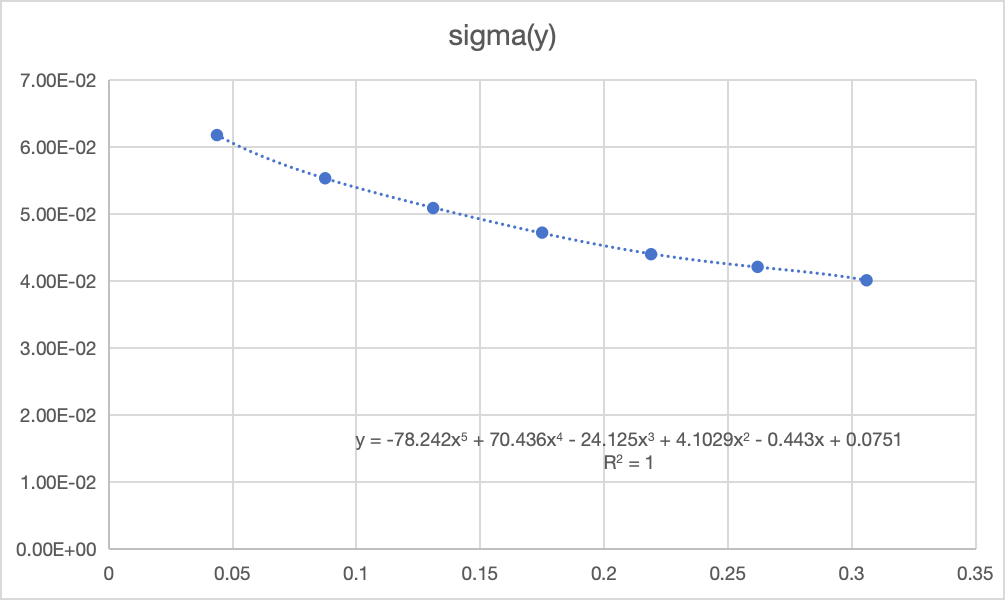
\includegraphics[width=1\textwidth]{fig1.png}
  \caption{pH-$\lg\frac{D-D_1}{D_2-D}$图}
  \label{fig1}
\end{figure}

\section{结果讨论}

由图\ref{fig1}可知\\
\begin{equation}
  \lg\frac{D-D_1}{D_2-D} = \text{pH}-\text pK_a=0.4363x+4.355
\end{equation}
因此
\begin{equation}
  \text pK_a=-4.355
\end{equation}
故
\begin{equation}
  K_a=10^{4.355}=\num{2.264e4}
\end{equation}


\section{误差来源}
误差与室温变化、恒温槽温度与室温温差变化、测量pH时溶液逐渐冷却、
所用HCl溶液挥发等有关.

\section{体会认识}
掌握了一种测定酸碱指示剂电离平衡常数的方法;
熟悉并掌握了722型分光光度计的性能和使用方法,并利用分光光度计测量BPB的最大吸收波长,了解溶液浓度对max的影响;
学会了用缓冲溶液调节溶液酸度的方法.~
